\Chapter{Tesztelés}

Ebben a fejezetben különböző szempontok alapján teszteljük az alkalmazást. Ebben segítségünkre lesz a \textit{Megvalósítás} fejezetében megemlített \textit{Postman} asztali alkalmazás. Fontos megjegyezni, hogy a szervergép tejlesítménye befolyásolja a program futásának sebességét!

%%%%%%%%%%%%%%%%%%%%%%%%%%%%%%%%%%%%%%%%%%%%%%%%%%%%%%%%%%%%%%%%%%%%%%%%%%%%%%%%%%%%%%%%%%%%%%%%%%%%%%%%%%%
%%%%%%%%%%%%%%%%%%%%%%%%%%%%%%%%%%%%%%%%%%%%%%%%%% 5 . 1 %%%%%%%%%%%%%%%%%%%%%%%%%%%%%%%%%%%%%%%%%%%%%%%%%%
%%%%%%%%%%%%%%%%%%%%%%%%%%%%%%%%%%%%%%%%%%%%%%%%%%%%%%%%%%%%%%%%%%%%%%%%%%%%%%%%%%%%%%%%%%%%%%%%%%%%%%%%%%%

\Section{A szerver indulása}

Első körben a \textit{package.json} fájlt kell létrehozni, mivel az alkalmazásunk ebben tárolja a fügőségeket (dependency-ket), ez alapján tölti be a szükséges modulokat. Ezt az \texttt{npm init} paranccsal tudjuk létrehozni. A folyamat kezdeményezése után átlagosan \textit{1 másodpercet (1000 ms)} kell várnunk, mire betölti a terminál a szükséges változókat. Ezután egyesével meg kell adnunk metaadatokat (például az alkalmazás neve, verziószáma, a szerző neve stb.). Miután megadtunk minden szükséges adatot, a terminál megjeleníti számunkra a legenerált tartalmat. Megerősítés után a tartalom kiírásra kerül a \textit{package.json} fájlba. A fájlba írás időtartama elhanyagolható.

A \textit{Node.js}-ről szóló részletben taglaltuk azt, hogyan tudjuk futtatni a programunkat. Ennek értelmében kiadjuk a \texttt{node <fajl>} parancsot a programozói felületünk terminálján, majd az alkalmazásunk betölti a szükséges adatokat, és futni kezd. Az ehhez szükséges időtartam változó. A szervergép indulása utáni első programindítás átlagosan \textit{5 másodpercet (5000 ms)} vesz igénybe, az ezt követő indításokhoz pedig átlagosan \textit{fél másodpercet (500 ms)} kell várnunk.

%%%%%%%%%%%%%%%%%%%%%%%%%%%%%%%%%%%%%%%%%%%%%%%%%%%%%%%%%%%%%%%%%%%%%%%%%%%%%%%%%%%%%%%%%%%%%%%%%%%%%%%%%%%
%%%%%%%%%%%%%%%%%%%%%%%%%%%%%%%%%%%%%%%%%%%%%%%%%% 5 . 2 %%%%%%%%%%%%%%%%%%%%%%%%%%%%%%%%%%%%%%%%%%%%%%%%%%
%%%%%%%%%%%%%%%%%%%%%%%%%%%%%%%%%%%%%%%%%%%%%%%%%%%%%%%%%%%%%%%%%%%%%%%%%%%%%%%%%%%%%%%%%%%%%%%%%%%%%%%%%%%

\Section{Felhasználói inputok szimulálása}

%%%%%%%%%%%%%%%%%%%%%%%%%%%%%%%%%%%%%%%%%%%%%%%% 5 . 2 . 1 %%%%%%%%%%%%%%%%%%%%%%%%%%%%%%%%%%%%%%%%%%%%%%%%

\subsection{Bejelentkezés szimulálása}

Az itt használatos változók:

\begin{itemize}
\item{\textbf{username}: a felhasználónevet tárolja}
\item{\textbf{password}: a jelszavat tárolja}
\end{itemize}

\newpage

\noindent{\textbf{\large{Nem létező felhasználónév}}}\\

Létrehozunk egy olyan szimulációt, melyben olyan nevű felhasználói fiókba próbálunk bejelentkezni, mely nem létezik. Ennek eredménye a \textit{"Felhasználó nem található!"} hibaüzenet (\ref{fig:loginNoUser}. ábra).

\begin{figure}[h]
	\centering
		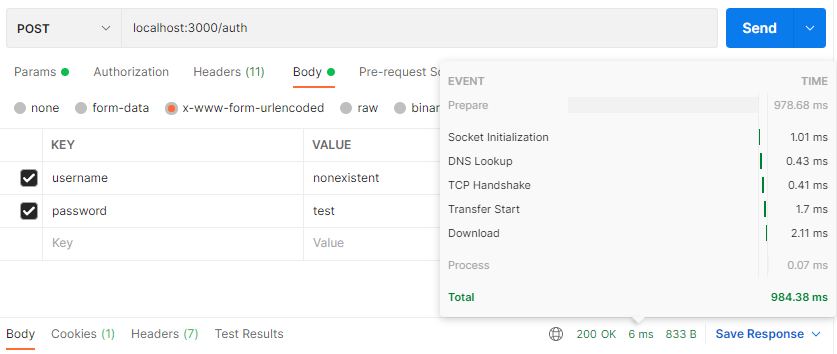
\includegraphics[width=15truecm, height=7truecm]{images/loginNoUser.png}
	\caption{A hibás nevű fiókba való bejelentkezés szimulációja}
	\label{fig:loginNoUser}
\end{figure}

\noindent{\textbf{\large{Hibás jelszó}}}\\

Ebben a folyamatban a felhasználói fiók neve már létezik az adatbázisban, viszont a hozzá kapcsolódó, illetve a felhasználó által begépelt (szimulált) jelszó nem egyezik. Ennek eredménye a \textit{"Helytelen jelszó!"} hibaüzenet (\ref{fig:loginBadPW}. ábra).

\begin{figure}[h]
	\centering
		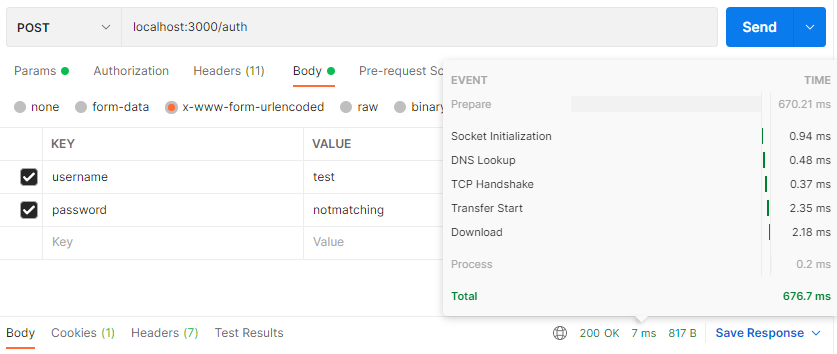
\includegraphics[width=15truecm, height=7truecm]{images/loginBadPW.png}
	\caption{A nem megfelelő jelszó szimulációja}
	\label{fig:loginBadPW}
\end{figure}

\noindent{\textbf{\large{Sikeres bejelentkezés}}}\\

A bejelentkezés utolsó szimulációjában egy sikeres login folyamatot mutatunk be. Ennek eredményeképp megjelenik a megfelelő (hallgatói vagy adminisztrátori) felület (\ref{fig:loginSuccess}. ábra).

\begin{figure}[h]
	\centering
		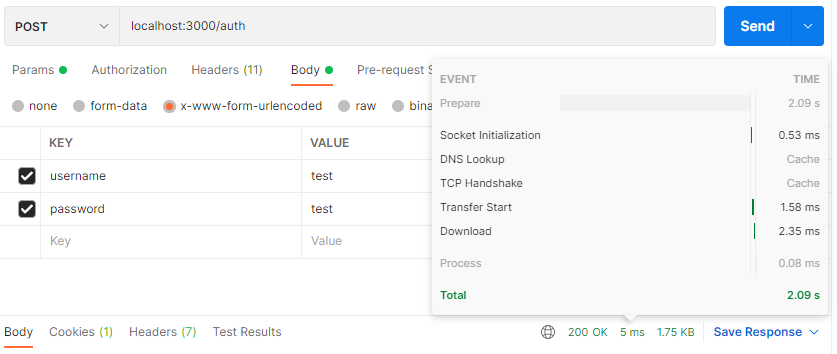
\includegraphics[width=15truecm, height=7truecm]{images/loginSuccess.png}
	\caption{A sikeres bejelentkezés szimulációja}
	\label{fig:loginSuccess}
\end{figure}

%%%%%%%%%%%%%%%%%%%%%%%%%%%%%%%%%%%%%%%%%%%%%%%% 5 . 2 . 2 %%%%%%%%%%%%%%%%%%%%%%%%%%%%%%%%%%%%%%%%%%%%%%%%

\subsection{Fájlfeltöltés szimulálása}

A fájlfeltöltés folyamatának szimulálásakor egyetlen változót használunk. Ez a \textit{fileUp}, mely tartalmazza a feltöltendő fájlt.\\

\noindent{\textbf{\large{Már létező fájl}}}\\

Először egy olyan fájlt próbálunk feltölteni, melynek neve már megtalálható a feltöltési mappában. Ebben az esetben a \textit{"Már létezik ilyen nevű fájl!"} visszajelzés jelenik meg (\ref{fig:uploadFileExists}. ábra).

\begin{figure}[h]
	\centering
		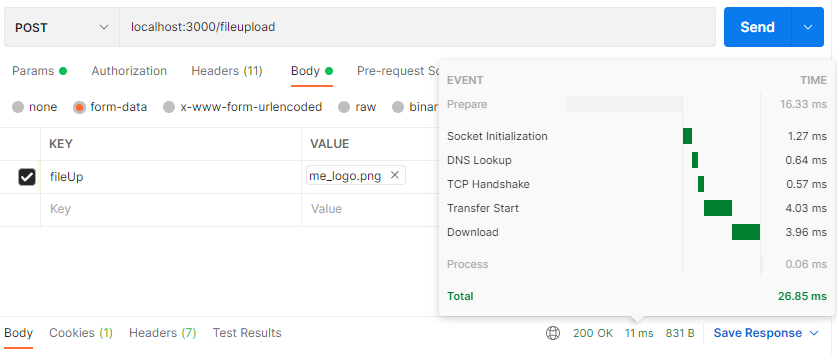
\includegraphics[width=15truecm, height=7truecm]{images/uploadFileExists.png}
	\caption{A nem egyedi nevű fájl feltöltésének szimulációja}
	\label{fig:uploadFileExists}
\end{figure}

\newpage

\noindent{\textbf{\large{Sikeres fájlfeltöltés}}}\\

A feltöltés második szimulációjában a sikeres folyamatot szimuláljuk. Ebben az esetben a \textit{"Sikeres fájlfeltöltés!"} üzenet jelenik meg (\ref{fig:uploadSuccess}. ábra).

\begin{figure}[h]
	\centering
		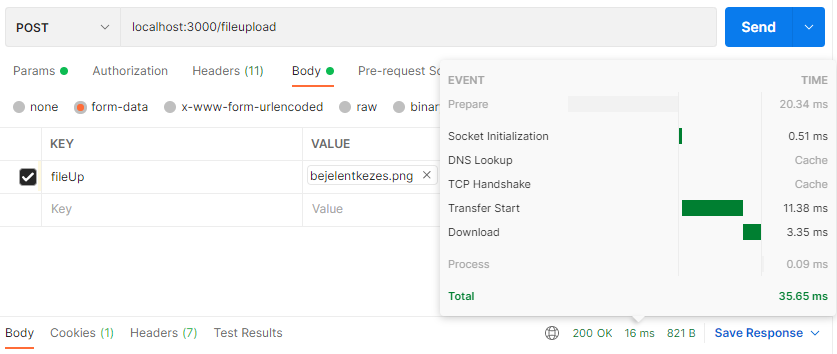
\includegraphics[width=15truecm, height=7truecm]{images/uploadSuccess.png}
	\caption{A sikeres fájlfeltöltés szimulációja}
	\label{fig:uploadSuccess}
\end{figure}

%%%%%%%%%%%%%%%%%%%%%%%%%%%%%%%%%%%%%%%%%%%%%%%% 5 . 2 . 3 %%%%%%%%%%%%%%%%%%%%%%%%%%%%%%%%%%%%%%%%%%%%%%%%

\subsection{Felhasználói fiók hozzáadásának szimulálása}

Végül egy adminisztrátori műveletet fogunk szimulálni, a felhasználó hozzáadásának folyamatát. Ehhez szükségünk lesz három változóra:

\begin{itemize}
\item{\textbf{addUName}: A felhasználónevet tároló változó}
\item{\textbf{addPW}: A jelszót tároló változó}
\item{\textbf{addPWAgain}: A jelszó ismételt begépelését tároló változó}
\end{itemize}

\noindent{\textbf{\large{Már létező felhasználó}}}\\

Először egy olyan felhasználót próbálunk hozzáadni az adatbázishoz, melynek neve már létezik. Ebben az esetben a \textit{"Már létezik ilyen nevű felhasználó!"} hibaüzenettel szembesülünk (\ref{fig:addUserExists}. ábra).

\begin{figure}[h]
	\centering
		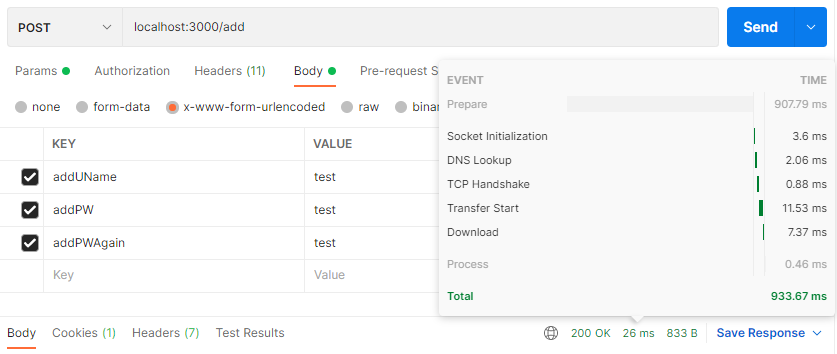
\includegraphics[width=15truecm, height=7truecm]{images/addUserExists.png}
	\caption{A nem egyedi nevű felhasználó hozzáadásának szimulációja}
	\label{fig:addUserExists}
\end{figure}

\newpage

\noindent{\textbf{\large{Nem egyező jelszavak}}}\\

A következő szimulációban olyan felhasználót próbálunk hozzáadni az adatbázishoz, melynek nem egyeznek a jelszavai. Ebben az esetben \textit{"A jelszavak nem egyeznek!"} hibaüzenettel szembesülünk (\ref{fig:addPWNotMatch}. ábra).

\begin{figure}[h]
	\centering
		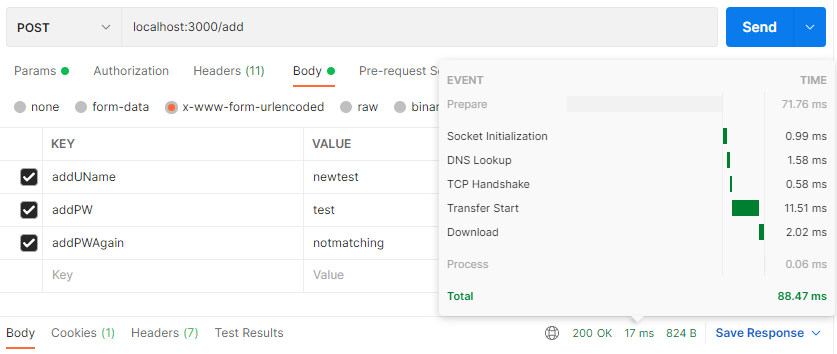
\includegraphics[width=15truecm, height=7truecm]{images/addPWNotMatch.png}
	\caption{A nem egyező jelszavú felhasználó hozzáadásának szimulációja}
	\label{fig:addPWNotMatch}
\end{figure}

\noindent{\textbf{\large{Sikeres felhasználói fiók hozzáadás}}}\\

Az utolsó szimulációban a sikeres fiók-hozzáadás folyamatát mutatjuk be. Ebben az esetben az \textit{"Adatbázis frissítése sikeres!"} üzenetet kapjuk (\ref{fig:addSuccess}. ábra).

\begin{figure}[h]
	\centering
		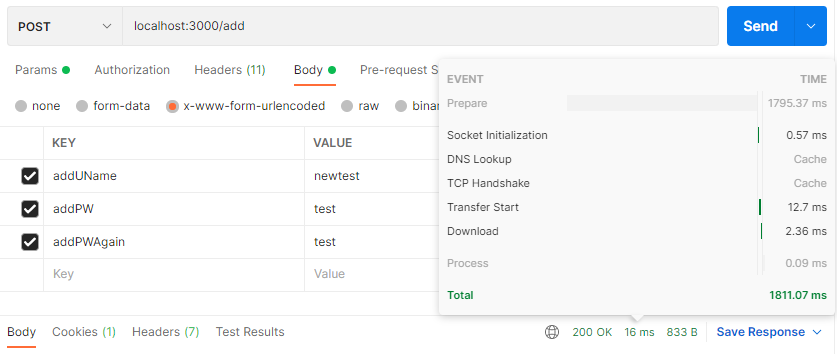
\includegraphics[width=15truecm, height=7truecm]{images/addSuccess.png}
	\caption{A felhasználó hozzáadásának sikeres szimulációja}
	\label{fig:addSuccess}
\end{figure}